\documentclass[10pt]{beamer}
\usepackage{tikz}
\tikzstyle{every node}=[circle, draw, fill=black!100, inner sep=0pt, minimum width=5pt]

\usepackage{amsthm}
\usepackage{amssymb}
\usepackage{amsmath}
\usepackage{graphicx}

\usepackage{mathrsfs}

\usepackage{lmodern}

%\usepackage[hang,scriptsize]{subfigure}

\usepackage[format=hang,font={scriptsize}]{caption}
\usepackage[format=hang,font={scriptsize}]{subcaption}

\usepackage{animate}
\usepackage{movie15}

%\usepackage{epsfig}
%\usepackage{tikz-3dplot}

%\usepackage{beamerthemesplit}

\usetheme{CambridgeUS}
\usecolortheme{beaver}

%\setbeamertemplate{footline}{}
%\setbeamertemplate{navigation symbols}{}
%\setbeamercovered{dynamic}
%\hypersetup{pdfpagemode=FullScreen}


\title[Statistical Mechanics Presentation]{Superconductors}
\author[W. Bowman]{\Large Wesley A. Bowman}
\institute{\Large Acadia University \\ \normalsize Physics Department}
%\titlegraphic{\includegraphics[width=20mm]{Acadia_logo}}


\hypersetup{pdfpagemode=FullScreen}
\setbeamertemplate{footline}[page number]{}
\setbeamertemplate{navigation symbols}{}
\setbeamertemplate{caption}[numbered]

\newtheorem{defn}{Definition}
\newtheorem{lem}{Lemma}
\newtheorem{thm}[lem]{Theorem}
\newtheorem{cor}[lem]{Corollary}

\theoremstyle{definition}
\newtheorem{ex}{Example}


\begin{document}

\begin{frame}
    \titlepage
\end{frame}

%%%%%%%%%%%%%%%%%%%%%%%%%%%%%%%%%%%%%%%%%%%%%%%%%%%%%%%%%%%%%%%%%%%%%%%%%%%%%%

\section{Introduction}
%\subsection{Introduction}
\begin{frame}
    \frametitle{Introduction}

    Superconductivity is defined as a complete disappearance of electrical
    resistance in a substance especially at very low temperatures.

    \begin{center}
    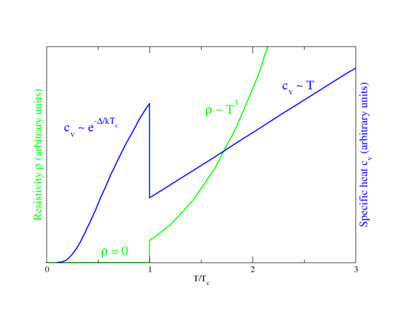
\includegraphics[scale=0.5]{tcSuperVsNormal.png}
    \end{center}

    Why does this happen?
    The flaws and vibrations of the atoms  in the materials should cause resistance in
    when the electrons flow through it,
    yet, the electric resistance is equal to
    zero although the flaws and vibrations still exist.

\end{frame}

\begin{frame}
    \frametitle{Electrons}

    Let's start with electrons, which are fermions. All fermions have
    half-integer spin. Now, because fermions have  to have the half-integer
    spin, we get a constraint on a system with more than one fermion
    \\~\\

    This constraint is called the Pauli exclusion principle, which states
    that no two fermions can have the exact same set of quantum numbers.
    \\~\\

    This causes electrons that have the same energy to have different spins,
    one having spin up and the other spin down, and why we can only have two
    electrons in each energy level.

\end{frame}

\begin{frame}
    \frametitle{Fermi-Dirac Distribution}

    Electrons are fermions and so at temperature $T$  and a state with
    energy $E$
    is occupied according to the Fermi-Dirac distribution:

    \begin{equation}
        f(\varepsilon) = \frac{1}{e^{\beta (E-\mu)}+1}
    \end{equation}
    where $f(\varepsilon)$ is the occupation probability of a state of
    energy $\varepsilon$, $\beta$ is $\frac{1}{k_B T}$, and $\mu$ is the
    chemical potential.
    \\~\\
    At absolute zero the value of the chemical potential is defined as the Fermi energy.
    At room temperature, it turns out the chemical potential for metals is
    virtually the same as the Fermi energy, with a typical different being on
    the oder of 0.01\%.



\end{frame}

\begin{frame}
    \frametitle{Superconductors}

    Things that make superconductors awesome and unique:
    \begin{itemize}
        \item
            Cooper Pairs
        \item
            Energy Gap
        \item
            Meissner Effect
    \end{itemize}

    All of which are gotten from the BCS theory.




\end{frame}

\begin{frame}
    \frametitle{ Bardeen, Cooper, and Schrieffer}

    BCS is the first theory that explained superconductivity at a microscopic scale. It also correctly predicts
the energy gap 2$\Delta$, twice the energy gap, at the fermi level.
\\~\\
It turns out that the effective forces between electrons can sometimes be attractive, this
is due to the phonon electron coupling. Cooper considered a single electron pair outside a occupied fermi
surface and found that the fermions formed a stable pair bound state no matter how weak the attractive
force. 
\\~\\

Schreiffer constructed a many particle wave function in which all electrons near the fermi
surface are paired up, this is a form of coherent states and the energy gap arises from it's analysis. 


\end{frame}


\begin{frame}
    \frametitle{Cooper Pairs}

    One electron passes by positively charged ions in the lattice of the
    superconductor, which makes the lattice distort.
    \\~\\

    In distorting an area of increased positive charge, the electron
    attracts a closely following negative electron that will also pass
    along the relatively positive trough in the distorted lattice area.
\\~\\

    The electron pairs produced in this way are coherent (in phase) as 
    they pass through the conductor in unison. The electrons are screened 
    by the phonons and, although paired, are separated by some distance.
\\~\\

%    When one of the electrons passes close to an ion in the crystal lattice, 
%    attraction between the negative electron and the positive ion occurs. This 
%    causes a vibration that passes from ion to ion in the crystal lattice 
%    until the other electron of the pair also absorbs the vibration. 

    This means that the first electron of the Cooper pair has emitted a 
    phonon and the second electron has absorbed that phonon.

%That exchange of energy somehow keeps the Cooper paired electrons together and in the same quantum state.


\end{frame}


\begin{frame}
    \frametitle{Cooper Pairs}

    As long as collisions with the ionic lattice of the solid do not supply 
    enough energy to break the Cooper pairs, the electron fluid will be able 
    to flow without dissipation. As a result, it becomes a superfluid, and the 
    material through which it flows a superconductor.

    \begin{center}
    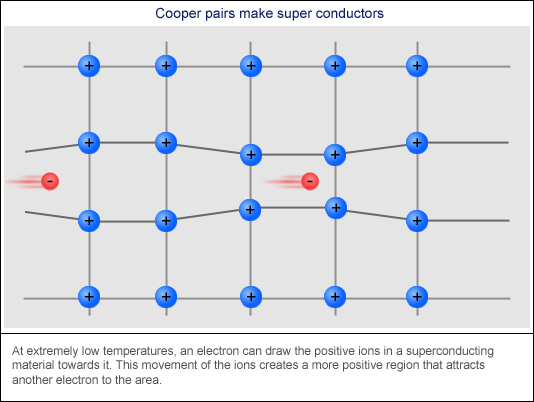
\includegraphics[scale = 0.3]{cooperpairs}
    \end{center}



\end{frame}


\begin{frame}
    \frametitle{Cooper Pairs}
%
%    When there is a flaw or when one of the atoms of the crystal pattern is vibrating, 
%    the wave is disrupted. At a very low temperature, the electrons pair up and merge 
%    into one quantum wave that fills the whole material. This unique wave becomes 
%    insensitive to the flaws in the material; they are too small to slow the whole wave. 
%    The electric resistance has hence disappeared.

    In a metal, electrons are waves. Each of these electrons is relatively independent 
    and follows its own path independent of other electrons. In a superconductor, 
    the majority of these electrons merge in order to form a large collective wave. 
    In quantum physics, we call it macroscopic quantum wavefunction, or condensate. 
    When the collective wave is formed, it requires each member to move at the same 
    speed. In a metal, an individual electron is easily diverted by a flaw or an atom 
    that is too big. In a superconductor however, this same electron can be diverted 
    only if, at the same time, all the other electrons of the collective wave are 
    diverted in the exact same manner. The flaw in a single atom surely cannot do 
    that; the wave will not be diverted, and, thus, not slowed down.



\end{frame}



\begin{frame}
    \frametitle{Energy Gap}

    The Cooper pairs are able to occupy lower energy-levels than the 
    electrons did and the spectrum 
    of energy levels contains a gap between the highest occupied 
    state and the next higher available state.
    \\~\\

    The pairs of electrons act more like bosons which can condense into the same 
    energy level. The electron pairs have a slightly lower energy and leave an 
    energy gap above them on the order of .001 eV which inhibits the kind of 
    collision interactions which lead to ordinary resistivity.
    \\~\\

    The essential point is that below $T_C$ the binding energy of a pair of
    electrons causes the opening of a gap in the energy spectrum at $E_F$, 
    separating the pair states from the normal single electron states.


\end{frame}

\begin{frame}
    \frametitle{Energy Gap}

    Excitations within the solid are not sufficient to overcome this gap 
    and so these paired electrons are able to travel through the solid 
    without interacting (scattering) off anything else present in the solid.
    \\~\\

    The BCS theory gives the expression of the energy gap that depends on 
    the Temperature $T$ and the Critical Temperature $T_C$ and is 
    independent of the material:

    \begin{equation}
        E_G = 3.52k_B T_C \left( 1-\frac{T}{T_{C}} \right)^{1/2}
    \end{equation}



\end{frame}


\begin{frame}
    \frametitle{Meissner Effect}

    When a material makes the transition from the normal to superconducting 
    state, it actively excludes magnetic fields from its interior; 
    this is called the Meissner effect.
    \\~\\
    It does this by setting up electric currents near its surface. 
    The magnetic field of these surface currents cancels the applied 
    magnetic field within the bulk of the superconductor. As the field 
    expulsion, or cancellation, does not change with time, the currents 
    producing this effect (called persistent currents) do not decay 
    with time.


\end{frame}


\begin{frame}
    \frametitle{Meissner Effect}

    This constraint to zero magnetic field inside a superconductor is 
    distinct from the perfect diamagnetism, which would arise from its 
    zero electrical resistance. Zero resistance would imply that if you 
    tried to magnetize a superconductor, current loops would be generated 
    to exactly cancel the imposed field (Lenz's law). But if the material 
    already had a steady magnetic field through it when it was cooled 
    through the superconducting transition, the magnetic field would be 
    expected to remain. If there were no change in the applied magnetic 
    field, there would be no generated voltage (Faraday's law) to drive 
    currents, even in a perfect conductor. Hence the active exclusion 
    of magnetic field must be considered to be an effect distinct from 
    just zero resistance.

    \begin{equation}
        \frac{d \phi}{dt} = 0
    \end{equation}
    The magnetic field remains constant as a function of time.

\end{frame}



\begin{frame}
    \frametitle{Type I or Type II}

    There are two types of superconductors, Type I and Type II.
    \\~\\

    When the magnetic field becomes too strong, the system becomes 
    a metal again. Type I superconductors demonstrate this type of behaviour.
    \\~\\

    Type II superconductors act a bit differently.
    Under a small magnetic field, they react like type I superconductors
    and completely expel the magnetic field. But when the magnetic field 
    is stronger, they prefer to adopt a compromise situation and allow 
    some of the magnetic field to penetrate along vortices. Each vortex is a
    small region in a superconductoring metal that acts like a normal metal.
    \\~\\

    The material then becomes a sieve. In order to enable this magnetic 
    field to go through the vortex, the material develops superconducting 
    currents circulating around this pillar in a spiral motion justifying 
    the name vortex.

%    \begin{center}
%    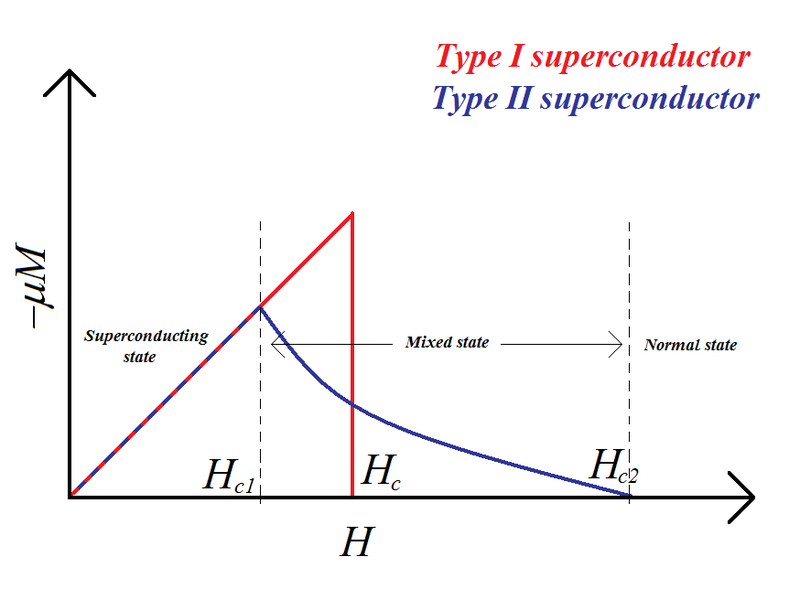
\includegraphics[scale = 0.3]{Magnetisation_and_superconductors}
%    \end{center}

\end{frame}




\begin{frame}
    \frametitle{Type I or Type II}

    \begin{center}
    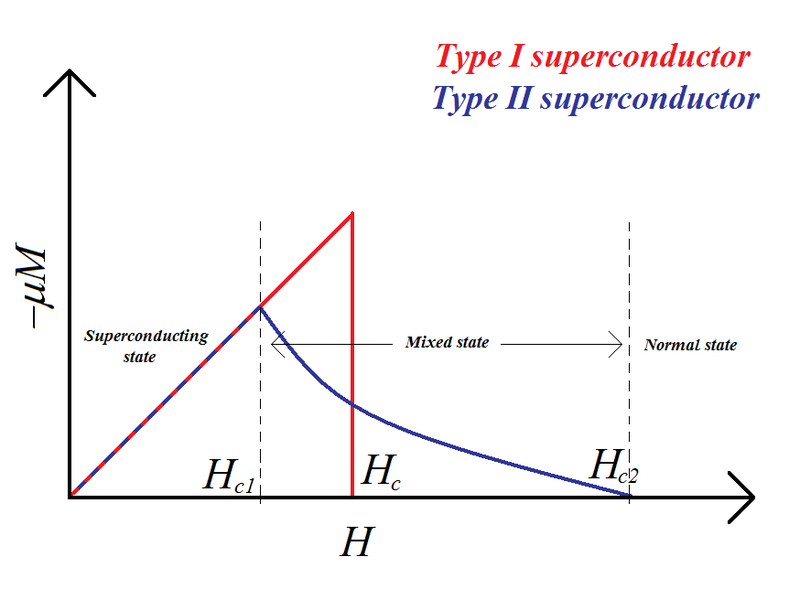
\includegraphics[scale = 0.3]{Magnetisation_and_superconductors}
    \end{center}

\end{frame}

\begin{frame}
    \frametitle{Conclusion}

    The key idea behind superconductors is that there is attraction between
    electron pairs, when normally we expect them to repulse one another. This
    gives us Cooper Pairs, which form the condensate (which can be thought of
    as a superfluid), that allows for an energy gap, and the zero resistivity.

\end{frame}

\begin{frame}
    \frametitle{Questions}

    Questions?


\end{frame}







\end{document}
